\documentclass{beamer}

\usepackage{amsmath}
\usepackage{bm}
\usepackage{amssymb}
\usepackage{tikz}
\usepackage{pgfplots}
\usepackage{hyperref}

\title{Quadratic Forms}
\subtitle{\(Q \colon \mathbb{R}^n \to \mathbb{R}\)}
\author{Ahmed Mohammed}
\institute{Georgia Institute of Technology}
\date{PLUS Session, Summer 2023}

\usetheme{Antibes}
\usefonttheme{serif}

% ------- Set up math stuff -------
\renewcommand{\vec}[1]{\bm{#1}}
\DeclareMathOperator{\vspan}{Span}
\DeclareMathOperator{\row}{row}
\DeclareMathOperator{\col}{col}
\DeclareMathOperator{\colspace}{Col}
\DeclareMathOperator{\nullspace}{Nul}
\DeclareMathOperator{\rank}{rank}
% -------------------------------------------------------

\hypersetup{
    colorlinks=true,
    linkcolor=blue,
    filecolor=magenta,      
    urlcolor=cyan,
    pdftitle={Quadratic Forms},
    pdfpagemode=FullScreen,
}

\AtBeginSection[]
{
    \begin{frame}
        \frametitle{Table of Contents}
        \tableofcontents[currentsection]
    \end{frame}
} % https://statisticaloddsandends.wordpress.com/2019/02/18/beamer-inserting-section-slides-before-each-section/

\begin{document}
	\begin{frame}
		\maketitle
	\end{frame}

	\section{Open Activity: Revision}
	\subsection{Quadratic Forms}
	\begin{frame}
		\frametitle{What is a Quadratic Form?}
		A \emph{quadratic form}:\pause
		\[Q \colon \mathbb{R}^n \to \mathbb{R}, \quad \vec{x} \mapsto \vec{x}^TA\vec{x},\] for some symmetric matrix 
		\(A \in \mathbb{R}^{n \times n}\). \pause
		
		\begin{exampleblock}{Question 1}
			What is the symmetric matrix \(A\) associated with the quadratic form \(Q(\vec{x}) = 3x^2_1 + 2x_3^2 + 2x_1x_2\)? What is the domain
			of \(Q\)?
		\end{exampleblock}
	\end{frame}
	
	\begin{frame}
		\frametitle{Types of Quadratic Forms}
		\begin{itemize}[<alert@+>]
			\item \textbf{Positive definite.} \(Q(\vec{x})  = 0 \iff \vec{x} = \vec{0}\) and \(\vec{x} \ne \vec{0} \implies Q(\vec{x}) > 0\).
			\item \textbf{Positive semi-definite.} \(\forall \vec{x} \in \mathbb{R}^n,\) \(Q(\vec{x}) \ge 0\).
			\item \textbf{Negative definite.} \(Q(\vec{x})  = 0 \iff \vec{x} = \vec{0}\) and \(\vec{x} \ne \vec{0} \implies Q(\vec{x}) < 0\).
			\item \textbf{Negative semi-definite.} \(\forall \vec{x} \in \mathbb{R}^n,\) \(Q(\vec{x}) \le 0\).
			\item \textbf{Indefinite.} Whatever doesn't belong in the previous four.
		\end{itemize}
	\end{frame}

	\begin{frame}
		\frametitle{Types of Quadratic Forms \tiny \textit{(Graphical Example)}}
		\[Q(\vec{x})  = 0 \iff \vec{x} = \vec{0} \ \text{and} \ \vec{x} \ne \vec{0} \implies Q(\vec{x}) > 0.\]
		\begin{figure}[!h]
			\centering
			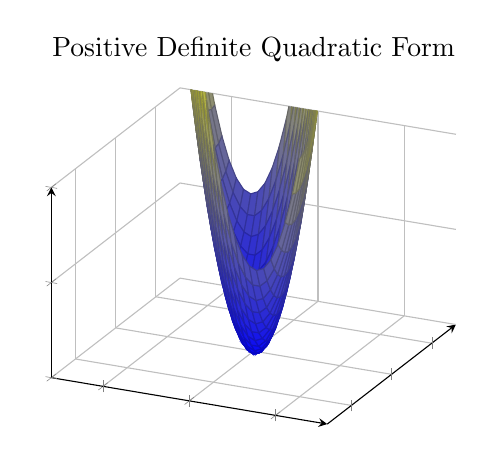
\begin{tikzpicture}
				\begin{axis}[
							axis lines = left, xticklabels=\empty, yticklabels=\empty, zticklabels=\empty,
							xmin=-8, xmax = 8, ymin=-8, ymax=8, zmin=0, zmax=10,
							title={Positive Definite Quadratic Form}, scale=0.75, grid=major
						  ]
					\addplot3[surf] {x^2 + 0.5*y^2 + x*y};
				\end{axis}
			\end{tikzpicture}
		\end{figure}
	\end{frame}

	\begin{frame}
		\frametitle{Types of Quadratic Forms \tiny \textit{(Graphical Example)}}
		\[\forall \vec{x} \in \mathbb{R}^n, \, Q(\vec{x}) \ge 0.\]
		\begin{figure}[!h]
			\centering
			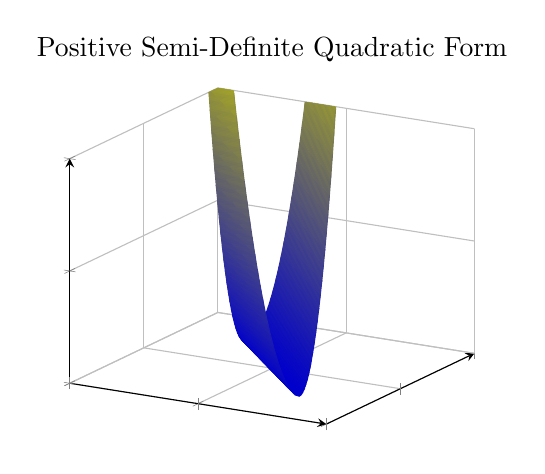
\begin{tikzpicture}
				\begin{axis}[
							axis lines = left, xticklabels=\empty, yticklabels=\empty, zticklabels=\empty,
							xmin=-10, xmax = 10, ymin=-10, ymax=10, zmin=0, zmax=10,
							title={Positive Semi-Definite Quadratic Form}, scale=0.75, grid=major, view={30}{20}
						  ]
					\addplot3[surf, samples=50] {0.5*x^2 + 0.5*y^2 + x*y};
				\end{axis}
			\end{tikzpicture}
		\end{figure}
	\end{frame}

	\begin{frame}
		\frametitle{Types of Quadratic Forms \tiny \textit{(Graphical Example)}}
		Look at \href{https://www.geogebra.org/m/c6det25z}{GeoGebra} for this graph.
	\end{frame}

	\begin{frame}
		\frametitle{Change Of Variables}
		Given that \(Q(\vec{x}) = \vec{x}^TA\vec{x},\) we can perform a \emph{change of variables} \(\vec{x} = P\vec{y}\) (where \(P\) is invertible) in 
		order to yield a new expression \(Q'(\vec{y}) = \vec{y}^TD\vec{y}.\) \pause

		\begin{exampleblock}{Question 2}
			Show that this is possible. Then, perform a change of variable on the quadratic form
			\(Q(\vec{x}) = \vec{x}^T\begin{bmatrix}2 & 1 \\ 1 & 2\end{bmatrix}\vec{x}\) so that we obtain a new quadratic form \(Q'\), where
			the matrix of \(Q'\) is a diagonal matrix. 
		\end{exampleblock}
	\end{frame}

	\subsection{Constrained Optimization}
	\begin{frame}
		\frametitle{Why Do We Care About Changing the Variables?}
		Performing a change of variables lead to simpler quadratic forms, ones that have no cross products. \pause
			\begin{itemize}[<+(1)->]
				\item Makes it easier to determine \emph{what} type of quadratic form we're dealing with.
				\item Makes it easier to determine \(\max_{\|\vec{x}\| = 1}\vec{x}^TA\vec{x}\) and \(\min_{\|\vec{x}\| = 1}\vec{x}^TA\vec{x}\).
					Also automatically allows for determining what inputs achieve these extreme outputs.
			\end{itemize}
		
		\onslide<5->{
		\begin{exampleblock}{Question 3}
			Continuing off the previous question, find the maximum and minimum of the quadratic form \(Q\) under the constraint \(\|\vec{x}\| = 1\),
			and find \emph{what inputs} yield those extreme values.
		\end{exampleblock}
		}
	\end{frame}

	\section{Main Activity}
	\begin{frame}
		\frametitle{Exercises}
		\textit{True, or false.} 
		\begin{itemize}[<+(1)->]
			\item Is it possible that the quadratic form \(Q(\vec{x}) = \vec{x}^TA^TA\vec{x}\) for any matrix \(A \in \mathbb{R}^{m \times n}\) is 
				indefinite?
			\item If the matrix of a quadratic form is diagonal, then the quadratic form has no cross product.
			\item For any quadratic form \(Q\), \(Q(c\vec{x}) = c^2Q(\vec{x}).\)
			\item The quadratic form \(Q \colon \mathbb{R}^n \to \mathbb{R}\) defined by \(Q(\vec{x}) = \vec{x}^TBB^T\vec{x}\) for any matrix \(B\)
				is always positive semi-definite.
			\item If \(A, B \in \mathbb{R}^{n \times n}\) are both positive definite symmetric matrices then the eigenvalues of \(A + B\) are positive.
		\end{itemize}

		\onslide<7->{
			What is the maximum and minimum value of \(Q(\vec{x}) = 5x_1^2 + 6x^2 + 7x^2_3 + 4x_1x_2 - 4x_2x_3\) under the constraint that
			\(\|\vec{x}\| = 1\) and where do those extreme values occur?
		}
		
	\end{frame}

	\section{Closing Activity}
	\begin{frame}
	\frametitle{SVD: MATH 1554's Closure}
		\centering \textit{Singular Value Decomposition.} \pause

		Takes everything we've learned, and puts it in a neat decompostion.
		\begin{itemize}[<+(1)->]
			\item Eigen-stuff.
			\item Orthogonality and orthonormal sets.
			\item The four fundamental subspaces.
			\item Bases.
			\item \textit{Singular values}. (This is new!)
		\end{itemize}
	\end{frame}
\end{document}